

%\documentclass[letterpaper, 10 pt, conference]{ieeeconf}  % Comment this line out if you need a4paper

\documentclass[a4paper, 10pt, conference]{ieeeconf}      % Use this line for a4 paper

\IEEEoverridecommandlockouts                              % This command is only needed if 
                                                          % you want to use the \thanks command

\overrideIEEEmargins                                      % Needed to meet printer requirements.

% See the \addtolength command later in the file to balance the column lengths
% on the last page of the document

% The following packages can be found on http:\\www.ctan.org
%\usepackage{graphics} % for pdf, bitmapped graphics files
%\usepackage{epsfig} % for postscript graphics files
%\usepackage{mathptmx} % assumes new font selection scheme installed
%\usepackage{times} % assumes new font selection scheme installed
%\usepackage{amsmath} % assumes amsmath package installed
%\usepackage{amssymb}  % assumes amsmath package installed
\usepackage{graphicx} 
\usepackage{amsmath}
\usepackage{bm}
\usepackage{leftidx}
\usepackage{hhline}
\usepackage{multirow}
\usepackage{epstopdf}

\usepackage[noadjust]{cite}
\title{\LARGE \bf
Stereo-Inertial Pose Estimation and Online Sensors 
Extrinsic Calibration
}


\author{Fumin Pang and Tianmiao Wang, \emph Member, \emph {IEEE}% <-this % stops a space
%\thanks{}% <-this % stops a space
\thanks{Fumin Pang and Tianmiao Wang are with the School of Mechanical Engineering and
	Automation, Beihang University, Beijing, 100191 China.
        {E-mail: fuminpang@buaa.edu.cn, itm@buaa.edu.cn}}%
}


\begin{document}



\maketitle
\thispagestyle{empty}
\pagestyle{empty}


%%%%%%%%%%%%%%%%%%%%%%%%%%%%%%%%%%%%%%%%%%%%%%%%%%%%%%%%%%%%%%%%%%%%%%%%%%%%%%%%
\begin{abstract}

The fusion of visual and inertial measurement has been popular in mobile robotics community for decades due to the complementary properties of two sensors. The combination of these two sensors offers rich  texture of environment and accurate short-time motion prediction, making it particularly suitable for pose estimation, especially in GPS-denied unknown environment. In this paper ,we propose a method which fuses stereo visual and inertial cues based on Multi-State Constraint Kalman Filter (MSCKF), to estimate 6DOF pose of mobile robot. Stereo vision offers real-metric perception of surroundings, giving a better initial scale estimation of the visual-inertial system. Compared with another class of methods based on batch nonlinear optimization , this filter-based method is more suitable for resource-constrained mobile platforms. In addition, the finite precision of sensors extrinsic calibration often makes estimator inconsistent. The proposed method includes extrinsic parameters in state vector to do online calibration. Experimental results on real-world datasets demonstrate that proposed method is consistent and substantially improves the accuracy of pose estimation, as well as the calibration between sensors.

\end{abstract}


%%%%%%%%%%%%%%%%%%%%%%%%%%%%%%%%%%%%%%%%%%%%%%%%%%%%%%%%%%%%%%%%%%%%%%%%%%%%%%%%
\section{INTRODUCTION}

Accurate 6DOF pose estimation in unknown environment is a critical component in autonomous navigation task. It is also one of the most popular topics in robotic community. Visual and inertial sensors have been more and more widely-applied to estimate the pose of mobile robots due to their complementary properties, low cost and safety. Visual measurement offers rich texture of surroundings. Each visual feature can always be tracked by a camera from a sequence  of consecutive poses, which provide  multiple constraint of camera motion. Inertial measurement can provide accurate motion prediction within a short time at  a higher frequency. In Simultaneous localization and mapping (SLAM), fusion of visual and inertial measurement is used to estimate robot pose and build a map of environment \cite{eade2006scalable} \cite{strelow2004motion}. Another pose estimation paradigm is Visual-Inertial Odometry (VIO),which merely  estimate robot motion typically.

In this paper, we are interested in visual-inertial odometry. The most common VIO methods can be classified into two categories: recursive filter-based and batch-based nonlinear optimization approaches. Filter-based approaches are the earlier ones used to solve SLAM and VIO problems. In this class of methods, inertial sensors are regarded as interoceptive sensors to provide linear accelerator and angular velocity, which are always integrated to form prior position and orientation estimation. Meanwhile,the visual sensors, as  exteroceptive sensors at a lower frequency,  provide visual measurement to calculate the innovation of the filter. Thus, posterior estimation is achieved recursively. Batch based methods are inspired by Structure From Motion (SFM) \cite{triggs1999bundle} and come into sight later, but achieve some impressing results in recent years \cite{leutenegger2015keyframe} \cite{strasdat2010scale} \cite{mur2015orb}. These methods promise results of higher accuracy compared with filtering approaches as they employ re-linearization at each iteration to get a better deal with the nonlinearity of the measurement models. They always implement bundle adjustment in a sliding window of states, using multiple iterations to minimize cost function, which results in increased computational cost, however. Thus, for a long-time running system,  the lack of computational resources mades recursive algorithms a favorable choice for online estimation, especially in resource-constrained systems, such as micro aerial vehicles, mobile phones, and Augmented Reality (AR) devices \cite{li2014visual}. Therefore, in this paper, we focus on the filter-based method.

Filter-based methods can also be divided into two main categories: loosely-coupled methods and tightly-coupled methods.Loosely-coupled ones are the most intuitive method for fusing visual and inertial measurement. This kind of methods deals with visual and inertial  measurement separately. Visual pipeline, always treated as a black box, estimate poses independently. These poses are regard as the measurement of EKF and then fused with the inertial measurement recursively \cite{kleinert2010inertial}. Weiss and Siegwart use a monocular  SLAM framework PTAM to estimate 6DOF poses of a micro aerial vehicle mounted with a down-looking camera \cite{klein2007parallel} \cite{weiss2011real} . Then, the poses are fused with the prior state vector driven by inertial reading. Lynen and Achtelik implement a EKF-based framework  for dealing  with loosely-coupled multiple sensor Fusion \cite{lynen13robust}. This kind of methods reduces computational complexity , but it will ignore some crucial information. For instance, processing IMU measurements separately does not allow for optimal estimation of sensor biases, and using feature measurements for motion estimation between pairs of images ignores the correlations between consecutive timesteps \cite{mourikis2007multi}.


Tightly-coupled methods are ones directly fuse the visual and inertial data for achieving higher precision. The most common EKF estimator to tightly fuse visual and inertial data is EKF-based SLAM, in which current camera pose and features positions are jointly included in estimator state vector \cite{jones2011visual} \cite{kelly2011visual}. EKF-based SLAM suffers from the cubic computational complexity of feature number in state  vector. To overcome this limitation, Mourikis and Roumeliotis come up with multi-state constraint Kalman filter(MSCKF) \cite{mourikis2007multi}. Instead of feature positions, a sliding window of camera poses is included in MSCKF estimator. By directly making use of the geometric constraints between multiple camera poses, it avoids the computational burden and loss of information associated with pairwise displacement estimation. To improve the consistency of the MSCKF, Li and Mourikis include Camera-IMU extrinsic calibration parameter in estimator state vector, giving a more accurate result \cite{li2013high}. 

In this paper, we propose a stereo visual inertial navigation system. As we know, almost all MSCKF-based implementations are based on monocular camera-IMU rig. Stereo visual measurement can give a real metric perception of   environment, which results in a better initialization of the estimator. A key contribution of proposed method is we give the derivation of stereo visual measurement model, which is different from the existing monocular one. In addition, to improve the performance, the system includes online extrinsic calibration between IMU and two cameras. We test the proposed method on real-world dataset. The experimental results show that the proposed method is consistent, and that it attains substantially higher accuracy than monocular MSCKF. And it gives a effective estimation about extrinsic parameters.


\section{ESTIMATOR DESCRIPTION}

As illustrated in Fig.1, we affix stereo camera-IMU rig body frame $\left\lbrace B \right\rbrace$ to IMU, to track the 6D motion with respect to a global coordinate frame, $\left\lbrace G \right\rbrace$.  Two camera coordinate frames, CAM0 and CAM1, are $\left\lbrace C_0 \right\rbrace$ and $\left\lbrace C_1 \right\rbrace$.




\subsection{MSCKF State Parametrization}
The full MSCKF state representation can be partitioned into three parts. The first is the evolving current body state. As we affix body frame $\left\lbrace B \right\rbrace$ to IMU, we use $ \textbf x_{I}  $ to present body state. We parametrize the body state at time \emph k as the 16-dimensional vector.

\begin {equation}
\textbf x_{I,k} :=\left[  {\leftidx{_G^B}{\bar{\textbf q}}_k}^{ T} \ \
{\leftidx{^G}{\textbf p}_{B,k}}^T \ \
{\leftidx{^G}{\textbf v}_{B,k}}^T \ \
\textbf b_{g,k}^T\ \
\textbf b_{a,k}^T 
\right]^T 
\end{equation}



Where $  {\leftidx{_G^B}{\bar{\textbf q}}_k}  $ is the unit quaternion representing the rotation which roatate vectors 
from the global frame  $\left\lbrace G \right\rbrace$ to the body frame  $\left\lbrace B \right\rbrace$. In this paper, all quaternions follow JPL convention \cite{sola2012quaternion}. $ {\leftidx{^G}{\textbf p}_{B,k}} $ is the vector from the
origin of $\left\lbrace G \right\rbrace$ to the origin of $\left\lbrace B \right\rbrace$ expressed in $\left\lbrace G \right\rbrace$ (i.e., the position of body in the global frame). $ {\leftidx{^G}{\textbf v}_{B,k}} $ is the vecotr repersenting original velocity of  frame  $\left\lbrace B \right\rbrace$ expressed in  $\left\lbrace G \right\rbrace$. $ \textbf b_{g,k} $ is the
bias on the gyro measurements $  \bm{ \omega}_m  $, $ \textbf  b_{a,k} $ is the bias on the
velocity measurements $ \textbf a_m $.

The second state part is extrinsic calibration parameters (rotation and translation) between IMU and two cameras. We parametrize it as a 14-dimensional vector.

\begin {equation}
\textbf x_{Calib,k} :=\left[  {\leftidx{_B^{C_0}}{\bar{\textbf q}}_k}^{ T} \ \
{\leftidx{^B}{\textbf p}_{C_0,k}}^T \ \
{\leftidx{_B^{C_1}}{\bar{\textbf q}}_k}^{ T} \ \
{\leftidx{^B}{\textbf p}_{C_1,k}}^T 
\right]^T
\end{equation}

Where $ {\leftidx{_B^{C_i}}{\bar{\textbf q}}_k} $ rotate vectors from body frame  $\left\lbrace B \right\rbrace$ to camera frame  $\left\lbrace C_i \right\rbrace$. $ {\leftidx{^B}{\textbf p}_{C_i,k}} $ is the original point position of camera frame  $\left\lbrace C_i \right\rbrace$ expressed in body frame  $\left\lbrace B \right\rbrace$, \emph i = 0,1.
\begin{figure}[thpb]
	\centering
	
	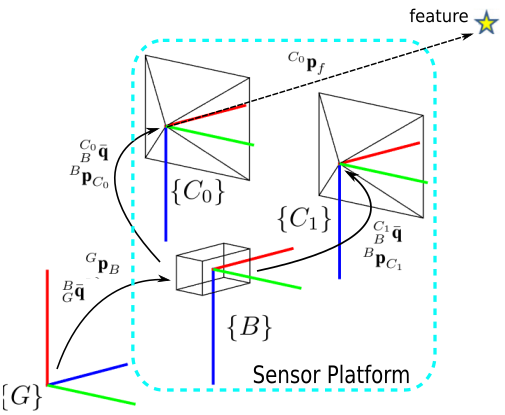
\includegraphics[scale=0.5]{frames2.png}
	
	\caption{Coordinate frames involved in sensor platform and visual feature.}
	\label{figurelabel}
\end{figure}

The third part of the full state is a sliding window of \emph N past body states, in which active feature tracks were visible. The \emph {i-th }body state, $ i = 0...N-1 $, inlcuding 6D pose and velocity, is a 10-dimensional vector. 
 
\begin {equation}
\textbf x_{B_i,k} :=\left[  {\leftidx{_{B_i}^{C_0}}{\bar{\textbf q}}_k}^{ T} \ \
{\leftidx{^B}{\textbf p}_{B_i,k}}^T \ \
{\leftidx{^G}{\textbf v}_{B_i,k}}^T
\right]^T
\end{equation}


At time \emph k, the full state of MSCKF is a (30 + 10* \emph N)  vector consisting of  current body state estimate, calibration parameters and \emph N 
last body states.

\begin {equation}
 \hat {\textbf x}_k :=\left[  {{\hat{\textbf x}}_{I,k}}^{ T} \ \
 {{\hat{\textbf x}}_{Calib,k}}^{ T} \ \
 {{\hat{\textbf x}}_{B_0,k}}^{ T}  \ \
 \ldots \ \
  {{\hat{\textbf x}}_{B_{N-1},k}}^{ T}  \ \
\right]^T
\end{equation}

We can  define \emph {error state} of the estimator  at time \emph k:
\begin {equation}
\tilde {\textbf x}_k :=\left[  {{\tilde{\textbf x}}_{I,k}}^{ T} \ \
{{\tilde{\textbf x}}_{Calib,k}}^{ T} \ \
{{\tilde{\textbf x}}_{B_0,k}}^{ T}  \ \
\ldots \ \
{{\tilde{\textbf x}}_{B_{N-1},k}}^{ T}  \ \
\right]^T
\end{equation}
where
\begin {equation}
\tilde{\textbf x}_{I,k} :=\left[  \leftidx{_B^G} { \bm {\delta \theta}}_{I}^T \ \
{\leftidx{^G}{\tilde {\textbf p}}_{B,k}}^T \ \
{\leftidx{^G}{\tilde {\textbf v}}_{B,k}}^T \ \
\tilde {\textbf  b}_{g,k}^T\ \
\tilde {\textbf b}_{a,k}^T 
\right]^T
\end{equation}
\begin {equation}
\tilde{\textbf x}_{B_i,k} :=\left[  \leftidx{_{B_i}^G} { \bm {\delta \theta}}_{I}^T \ \
{\leftidx{^G}{\tilde {\textbf p}}_{B_i,k}}^T \ \
{\leftidx{^G}{\tilde {\textbf v}}_{B_i,k}}^T \ \
\right]^T
\end{equation}
The full error state has  (27 + 9 \emph N) dimensions. In the above, $ \tilde x $ is the difference between the true value $ x $ and the estimated
value $ \bar x $. For position, velocity and bias, it is definde as $ \tilde x  = x - \bar x $. The quaternion error is definde  according to 
\begin {equation}
\bm { \delta {\bar q}} := \bm{\hat{\bar q}}^{-1} \otimes \bm {  {\bar q}} \approx \left[\frac{1}{2}{ \bm {\delta \theta}}^T  \ \ 1\right]^T
\end{equation}
Accordingly, the MSCKF error state covariance $ \bm{P} $ is a (27 + 9 \emph N) $ \times $ (27 + 9 \emph N) matrix. It can be partitioned into 4 blocks:
\begin{equation}
\bm{P} = \left[  \begin{matrix} 
\bm{P_{I,I}}  &\bm{P_{I,Cali-B}}  \\
\bm{P_{I,Cali-B}}^T & \bm{P_{Cali-B,Cali-B}}  \\
\end{matrix}   \right] 
\end{equation}
where $ \bm{P_{I,I}} $ is the $ 15 \times 15 $ covariance matrix of current body state.$  \bm{P_{Cali-B,Cali-B}}$ is the combinated $ (12 + 9 \emph N) \times (12 + 9 \emph N )  $   covarince matrix of calibration state and past body states. $\bm{P_{I,Cali-B}}  $ is the cross-covariance
between the current body  state and combination of calibration and past body states.
  


\subsection{Filter Propagation}

The IMU measurement is used to propagate the state estimates. As mentioned before, IMU measurement provide rotational velocity $ \bm {\omega}_m $ and $ \bm a_m $, described as below equations: 
\begin{equation}
\bm{\omega}_m ={\leftidx{^G}{ {\bm \omega}}_{}} + \bm b_g + \bm n_g
\end{equation}
\begin{equation}
\bm{a}_m =   \leftidx{_G^B}{{\textbf R}}  \left( \leftidx{^G}{\bm a} - \leftidx{^G}{\bm g}\right) + \bm b_a +\bm n_a
\end{equation}
where $ \leftidx{_G^B}{{\textbf R}} $ is the rotation matrix cooresponding to $  \leftidx{_G^I}{{\textbf q}} $. $\leftidx{^G}{\bm g}  $ is the gravitational acceleration.  $ \bm n_g $ and $ \bm n_a $  are zero-mean white Gaussian noise vectors. Using these measurements, we can
write the dynamics of the filter state vector as:
\begin{equation}
\leftidx{_G^I}{\dot {\bar{\textbf q}}}(t)=\frac{1}{2} \bm \Omega\left(  {\bm \omega}_m (t)-\bm b_g(t) - \bm n_g(t) \right)\leftidx{_G^I}{ {\bar{\textbf q}}} 
\end{equation}
\begin{equation}
{\leftidx{^G}{\dot {\textbf v}}_{B}}(t)=\leftidx{_G^B}{{\textbf R}}^T(t)\left( \bm a_m(t)-\bm b_a(t)-\bm n_a(t) \right)+  \leftidx{^G}{\bm g}
\end{equation}
\begin{equation}
{\leftidx{^G}{\dot {\textbf p}}_{B}}(t)= {\leftidx{^G}{ {\textbf v}}_{B}}(t)
\end{equation}
\begin{eqnarray}
{ \bm {\dot b_g}}(t) =  \bm n_{wg}(t) & { \bm {\dot b_a}}(t) =  \bm n_{wa}(t)
\end{eqnarray}
\begin{eqnarray}
\leftidx{_B^{C_i}}{\dot {\bar{\textbf q}}}(t) = \bm 0 & \leftidx{^B}{\dot {{\textbf p}}}_{C_i}(t)= \bm 0
\end{eqnarray}
where $ \bm \Omega $ is the quaternion multiplication matrix corresponding to the angular velocity vector $ \bm \omega $. In the above, the first three equations describe the dynamics of the current body motion. The fourth line models the biases  as random walk processes. The fifth line describes the fact that camera-IMU transformations do not change in time. As for the past body states, they remain constant once the corresponding image is captured.

Equation ($12$)-($16$) describe the the continuous-time evolution of the true states. 
We follow the approach described in  ( High-precision, consistent EKF-based visual-inertial odometry) for propagating the state estimates in a discrete-time implementation. Further, a fifth-order
Runge-Kutta procedure is used for propagate quaternion.

 Besides the current body position, velocity, and orientation, all other state estimates remain unchanged during propagation. We can also examine the linearized continuous-time model of the current state error state, $ {{\tilde{\textbf x}}_{I}} $:
\begin{equation}
{\dot{\tilde{\textbf x}}_{I}} =  \bm F{\tilde{\textbf x}}_{I}+\bm G \bm n_I
\end{equation}
where $ \bm F $ is the continuous-time error-state transition matrix. G is given by
\begin{equation}
\bm G = \left[\begin{matrix}  
- \bm {I_{3}} & \bm {0_{3}} & \bm {0_{3}} &\bm {0_{3}} \\
\bm {0_{3}} & \bm {0_{3}} & \bm {0_{3}} &\bm {0_{3}} \\
\bm {0_{3}} & - \bm {\leftidx{_G^B}{\hat {\textbf R}}^T} & \bm {0_{3}} &\bm {0_{3}} \\
\bm {0_{3}} & \bm {0_{3}} & \bm {I_{3}} &\bm {0_{3}} \\
\bm {0_{3}} & \bm {0_{3}} & \bm {0_{3}} &\bm {I_{3}} 
\end{matrix}  \right] 
\end{equation}
and $ \bm n_I = [\bm n_g^T \ \bm n_{a}^T \  \bm n_{wg}^T \ \bm n_{wa}^T]^T $ is the IMU process noise, which has covarince matrix $ \bm Q_I $.

In addition to the state estimate, the MSCKF propagates the state covariance matrix, as follows:

\begin{equation}
\bm{P}(t_{k+1})= \left[  \begin{matrix} 
\bm{P_{I,I}}(t_{k+1})  & 
\bm {\Phi}_{I_k}\bm{P_{I,Cali-B}}(t_{k+1}) \\
\bm{P_{I,Cali-B}}^T(t_k) \bm {\Phi}_{I_k}^T & \bm{P_{Cali-B,Cali-B}}(t_k)  \\
\end{matrix}   \right] 
\end{equation}
where
\begin{equation}
\bm{P_{I,I}}(t_{k+1})= \bm {\Phi}_{I_k}\bm{P_{I,I}}(t_{k}) \bm {\Phi}_{I_k}^T+\bm {G{Q_I}G^T\Delta T}
\end{equation}
and $ \bm {\Delta T} $ is the IMU sample period. $ \bm {\Phi}_{I_k} $ is the discrete-time error-state transition matrix at \emph k . Instead of using the most common approximation $ \bm \Phi = \bm I + \bm F\bm {\Delta T} \ $, we use the closed-form matrix by \cite{li2013high}.

\subsection{State Augmentation}
Upon recording a new image, a copy of current body rotation, position and velocity is appended
to the state vector, and the covariance matrix of the MSCKF is augmented accordingly:
\begin{equation}
\bm{P}(t_k) \leftarrow \left[ \begin{matrix}  \bm {I_{27+9N}} \\  \bm J \end{matrix}  \right]  \bm{P}(t_k)\left[ \begin{matrix}  \bm {I_{27+9N}} \\  \bm J \end{matrix}  \right]^T
\end{equation}
where J is given by 
\begin{equation}
\bm J = \left[ \begin{matrix}  \bm {I_{3}} & \bm {0_{3}} & \bm {0_{3}} & \bm {0_{3 \times {(18+9N)}}} \\ 
  \bm {0_{3}} & \bm {I_{3}} & \bm {0_{3}} & \bm {0_{3 \times {(18+9N)}}} \\ 
   \bm {0_{3}} & \bm {0_{3}} & \bm {I_{3}} & \bm {0_{3 \times {(18+9N)}}} 
   \end{matrix}  \right] 
\end{equation}

\subsection{Filter Update}
When a tracked feature $ \bm {f_j} $ is lost in current frame, it is selected for state update, the MSCKF estimates its position  $  \leftidx{^G}{\hat {\textbf p}_f} $ using an inverse depth \cite{montiel2006unified} least-squares Gauss-Newton optimization \cite{hartley2003multiple}. The procedure takes as input N pair of camera pose and N sets of feature measurements. As for stereo visual system , each past body pose has two corresponding camera poses, and the two camera poses can be calculated by 
\begin{equation}
 \leftidx{_G^{C_i}}{{\hat {\bar {\textbf q}}}}=   \leftidx{_B^{C_i}}{{\hat {\bar {\textbf q}}}} \otimes
 \leftidx{_G^{B}}{{\hat {\bar {\textbf q}}}}  \ \ \  {\leftidx{^G}{\textbf p}_{C_i}} =  {\leftidx{^G}{\textbf p}_{B}}+ \leftidx{_G^B}{\hat {\textbf R}}^T{\leftidx{^B}{\textbf p}_{C_i}} 
\end{equation}
Now that we have estimated the positions of any features
which can be used in the state update, we can apply the corresponding motion constraints to the window of poses from which each feature was tracked. To present the measurement model, we consider one feature,$ \bm f_j $, which is observed by a set of pose pairs, $ \mathcal M_j $. $ \bm z_{l,0} $ and $ \bm z_{l,1} $  are observations of feature $ \bm f_j $ from  stereo camera poses $ \bm C_{l,0} $ and $ \bm C_{l,1}$, $ l \in \mathcal M_j $. The $ 4 \times 1 $ stereo visual  measurement residual can be computed by
\begin{equation}
\bm {r}_l^{(j)} = \left[ \begin{matrix} \bm z_{l,0}^{(j)} \\ \bm z_{l,1}^{(j)} \end{matrix}\right] - \left[ \begin{matrix} \bm {\hat z}_{l,0}^{(j)} \\ \bm {\hat z}_{l,1}^{(j)} \end{matrix}\right] 
\end{equation}
where
\begin{equation}
 \bm {\hat z}_{l,i}^{(j)} = \frac{1}{\leftidx{^{C_{l,i}}}{\bm {\hat Z}}^{(j)}}\left[ \leftidx{^{C_{l,i}}}{\bm {\hat X}}^{(j)} \ \ \leftidx{^{C_{l,i}}}{\bm {\hat Y}}^{(j)} \right]^T
\end{equation}
with 
\begin{equation}
\begin{split}
{\leftidx{^{C_{l,i}}}{\bm{\hat p} }_{f_j}}& =  \left[ \leftidx{^{C_{l,i}}}{\bm {\hat Z}}^{(j)} \  \leftidx{^{C_{l,i}}}{\bm {\hat X}}^{(j)} \  \leftidx{^{C_{l,i}}}{\bm {\hat Y}}^{(j)} \right]^T \\
& =  \leftidx{_G^{C_{l,i}}}{\bm {\hat R}}\left({\leftidx{^{G}}{\bm {\hat p} }_{f_j}}-{\leftidx{^{G}}{\bm {\hat p}}_{C_{l,i}}} \right) 
\end{split}
\end{equation}






Linearizing about the estimates for the body pose and
for the feature position, the residual of Eq. $ (24) $ can be approximated as:
\begin{equation}
\bm {r}_l^{(j)} =\bm{H_{x_{B_l}}^{(j)}}{\tilde {\bm x}}+\bm{H_{f_{l}}^{(j)}}{\leftidx{^{G}}{\bm {\tilde p}}_{f_{j}}}+{\bm n_l^{(j)}}
\end{equation}
where the matrices $ \bm{H_{x_{B_l}}^{(j)}} $ and $ \bm{H_{f_{l}}^{(j)}} $ are the corresponding Jacobians of the measurement $  \bm {\hat z}_{l}^{(j)} $ with respect to the state and the
feature position, respectively, and $ {\leftidx{^{G}}{\bm {\tilde p}}_{f_{j}}} $ is the error in the
position estimate of $ \bm f_j $. $ \bm n_l^{(j)} $ is the $ 4 \times 1 $ visual measurement noise with the corresponding  covariance matrix  $ \bm R_l^{(j)} = {\sigma}_{im}^2 \bm I_4 $. $ \bm{H_{x_{B_l}}^{(j)}} $ is given by
\begin{equation}
 \bm{H_{x_{B_l}}^{(j)}}=\left[\begin{matrix} \bm 0_{4 \times 15} & \bm {\Pi}_l & \bm 0_{4 \times 9(l-1)} & \bm H_{B_l} & \bm 0_{4 \times 9(N-l)}
 \end{matrix} \right] 
\end{equation}
where
\begin{equation}
\bm {\Pi}_l =\left[\begin{matrix}
 \bm {\Pi}_{\bm {\theta}_{l,0}} & \bm {\Pi}_{\bm {p}_{l,0}} & \bm 0_{2 \times 3}  & \bm 0_{2 \times 3} \\ 
  \bm 0_{2 \times 3}  & \bm 0_{2 \times 3} & \bm {\Pi}_{\bm {\theta}_{l,1}} & \bm {\Pi}_{\bm {p}_{l,1}} 
\end{matrix} \right] 
\end{equation}
\begin{equation}
\bm H_{B_l} =\left[\begin{matrix}
 \bm {H}_{\bm {\theta}_{l,0}} & \bm {H}_{\bm {p}_{l,0}} & \bm 0_{2 \times 3}\\ 
  \bm {H}_{\bm {\theta}_{l,1}} & \bm {H}_{\bm {p}_{l,1}} & \bm 0_{2 \times 3}
\end{matrix} \right] 
\end{equation}
and for more details,the nonzero blocks in matrixs are  the Jacobians with respect to  the two camera-IMU rotations ,camera-IMU translations,  body rotation  and body position , respectively:
\begin{align}
&\bm {\Pi}_{\bm {\theta}_{l,i}} = \bm J_l^{(j,i)} \leftidx{_B^{C_i}}{\hat {\textbf R}}  \lfloor \leftidx{_G^B}{\hat {\textbf R}} (\leftidx{^{G}}{\bm { p}}_{f_{j}}-\leftidx{^{G}}{\bm {\tilde p}}_B)\times \rfloor \\ 
&\bm {\Pi}_{\bm {p}_{l,i}}  = \bm J_l^{(j,i)} \\
& \bm {H}_{\bm {\theta}_{l,i}}  = \bm J_l^{(j,i)}  \leftidx{_B^{C_i}}{\hat {\textbf R}} \leftidx{_G^B}{\hat {\textbf R}} \lfloor (\leftidx{^{G}}{\bm { p}}_{f_{j}}-\leftidx{^{G}}{\bm {\tilde p}}_B)\times \rfloor \\ 
& \bm {H}_{\bm {p}_{l,i}}  = -\bm J_l^{(j,i)} \leftidx{_B^{C_i}}{\hat {\textbf R}} \leftidx{_G^B}{\hat {\textbf R}}
\end{align}
where $ \lfloor \bm c\times \rfloor  $ is the skew symmetric matrix corresponding to vector $ \bm  c $. And $ \bm{H_{f_{l}}^{(j)}} $ is given by 
\begin{equation}
\bm{H_{f_{l}}^{(j)}} =  \bm J_l^{(j,i)} \left[\begin{matrix} \leftidx{_B^{C_0}}{\hat {\textbf R}} \leftidx{_G^B}{\hat {\textbf R}} \\  \leftidx{_B^{C_1}}{\hat {\textbf R}} \leftidx{_G^B}{\hat {\textbf R}} \end{matrix}  \right]  
\end{equation}
In the above, $ \bm J_l^{(j,i)} $ is the Jacobian of the perspective model:
\begin{equation}
\bm J_l^{(j,i)}=  \frac{1}{\leftidx{^{C_{l,i}}}{\bm {\hat Z}}^{(j)}}\left[ \begin{matrix} \bm 1 & \bm 0 &\dfrac{\leftidx{^{C_{l,i}}}{\bm {\hat X}}^{(j)}}{\leftidx{^{C_{l,i}}}{\bm {\hat Z}}^{(j)}} \\ \bm 0 & \bm 1 & \dfrac{\leftidx{^{C_{l,i}}}{\bm {\hat Y}}^{(j)}}{\leftidx{^{C_{l,i}}}{\bm {\hat Z}}^{(j)}} \end{matrix} \right]
\end{equation}
Stacking the residuals
of all $  \mathcal M_j  $measurements of this feature, we can get:
\begin{equation}
\bm {r}^{(j)} =\bm{H_{x_{B}}^{(j)}}{\tilde {\bm x}}+\bm{H_{f}^{(j)}}{\leftidx{^{G}}{\bm {\tilde p}}_{f_{j}}}+{\bm n^{(j)}}
\end{equation}
where $ \bm {r}^{(j)} $, $ \bm{H_{x_{B}}^{(j)}} $, $ \bm{H_{f}^{(j)}} $, and $ {\bm n^{(j)}} $ are block vectors or matrices with elements $ {r}_l^{(j)} $ , $ \bm{H_{x_{B_l}}^{(j)}} $, $ \bm{H_{f_{l}}^{(j)}} $, and $ {\bm n_l^{(j)}} $, for  $ \bm l \in \mathcal M_j $. And   $  \bm R_l^{(j)} = {\sigma}_{im}^2 \bm I_{4\mathcal M_j} $.
Eq.(37)  can not be directly used for measurement update in MSCKF. Because the term $ \bm{H_{f}^{(j)}}{\leftidx{^{G}}{\bm {\tilde p}}_{f_{j}}} $ is not part of state vector. In order to transform Eq.(37) into a standard form for update, we can compute a semi-unitary matrix $ \bm A $ whose columns form
the basis of the left nullspace of $ \bm{H_{f}^{(j)}} $, and multiply both sides of Eq.(37) by $ \bm A $ .

\begin{figure}[thpb]
	\centering
	
	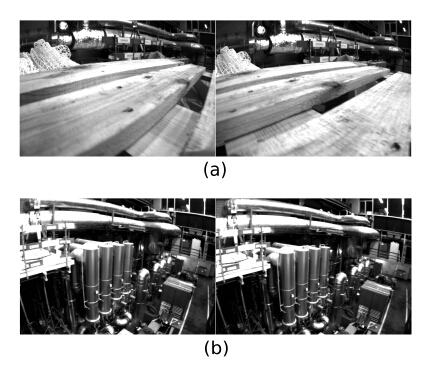
\includegraphics[scale=0.7]{sample.jpg}
	
	\caption{Sample images from dataset used in pose estimation experiment. (a) is the first pair of stereo images. (b) is the last pair. }
	\label{figurelabel}
\end{figure}

\begin{equation}
\begin{split}
\bm {r_o}^{(j)} = \bm A^T\bm {r}^{(j)} & =\bm A^T \bm{H_{x_{B}}^{(j)}}{\tilde {\bm x}}+\bm 0+ \bm A^T{\bm n^{(j)}} \\
& = \bm{H_{o}^{(j)}}{\tilde {\bm x}} + {\bm n_0^{(j)}}
\end{split}
\end{equation}
Now , we obtain the useful form for filter update. 
 $ \bm{H_{x_{B}}^{(j)}} $ has full column rank, accordingly, A has dimension $  4 \mathcal M_j \times
(4 \mathcal M_j-3)  $ and  $ \bm {r_o}^{(j)}  $ has dimension $ (4 \mathcal M_j-3) \times 1 $. The
covariance matrix of $ {\bm n_o^{(j)}} $ is  $ \bm {R_o}^{(j)}  = \bm A^T{\bm R^{(j)}}\bm A $.
We can now stack all the errors $ \bm {r_o}^{(j)}  $ for all the features selected for update.
\begin{equation}
\bm {r_o}= \bm{H_o}{\tilde {\bm x}} + {\bm n_o}
\end{equation}
To reduce the
computational complexity of the MSCKF update, a QR-decomposition of $ \bm{H_o} $ is employed.
\begin{equation}
\bm {H_o}= \left[\begin{matrix} \bm Q_0 \ \ \bm Q_1\end{matrix} \right] \left[\begin{matrix} \bm H_T \\ \bm 0\end{matrix} \right] 
\end{equation}
where $ \bm Q_0 $, $ \bm Q_1 $ are unitary matrices and $ \bm H_T $ is an uppertriangular matrix. Substituting this result into (39) , we obtain:
\begin{equation}
\left[\begin{matrix} \bm Q_0^T \bm r_o \\ \bm Q_1^T\bm r_o\end{matrix} \right]=  \left[\begin{matrix} \bm H_T \\ \bm 0\end{matrix} \right] {\tilde {\bm x}} + \left[\begin{matrix} \bm Q_0^T \bm n_0 \\ \bm Q_1^T\bm n_0\end{matrix} \right] 
\end{equation}
We discard term $ \bm Q_1^T\bm r_o $ ,because it is only noise. And we re-define error term used for update:
\begin{equation}
\bm {r_n}:=\bm Q_0^T \bm r_o =\bm{H_T}{\tilde {\bm x}} + \bm Q_0^T \bm n_0 =\bm{H_T}{\tilde {\bm x}} + \bm n_n
\end{equation}



Then, the covariance matrix of n
n is $ \bm R_n = \bm Q_0^T \bm R_o \bm Q_0 $.
Now, we arrive at  the final form of measurement equation. We can finally  formulate the Kalman gain and correction
equations to obtain the updated estimates for the filter state and covariance:
\begin{align}
\bm K &= \bm P_{k+1}\bm H_T^T																		(\bm H_T \bm P_{k+1} \bm H_T^T + \bm R_n )^{-1} \\
 \bm {x}_{k+1} &  \leftarrow  \bm {x}_{k+1} + \bm K \bm r_n \\
  \begin{split}
  \bm P_{k+1} &  \leftarrow (\bm I_{27+9N}-\bm K \bm H_T) \bm
  P_{k+1}(\bm I_{27+9N}-\bm K \bm H_T)^T \\
 & \ \ \ \ +\bm K \bm R_n \bm K^T
  \end{split}
\end{align}


	
\section{EXPERIMENTS}

We tested the proposed method and compared it with the monocluar-based MSCKF method on the  EuRoC MAV dataset recorded by ETH Autonomous Systems Lab. This dataset is recorded using VI-sensor and includes data streams from stereo camera and IMU \cite{Burri25012016}. The carefully calibrated extrinsic parameters and millimeter accurate position ground-truth is available in this dataset.
 
We implemented and tested both algorithms in MATLAB
2014b on a Lenovo laptop with a 2.4 GHz
Intel Core i7 processor and 12 GB of DDR3L RAM. We extracted between 100 and 200 salient point features  using Oriented FAST and Rotated BRIEF (ORB) detector \cite{rublee2011orb} of OpenCV \cite{opencv_library} from the stereo pairs and tracked them temporally using Kanade-Lucas-Tomasi (KLT) tracking \cite{birchfield2007klt}.  Outliers are rejected 
using a 5-point  Random Sample Consensus (RANSAC) . We conducted two experiments on the dataset to compare the accuracy of the the proposed method with the monocular-based one and show the result of the calibration between sensors. We will discuss both of these in turn.



\subsection{Pose Estimation} 

To compare the performance between monocular-based MSCKF (m-MSCKF) and the proposed method, we implemented a m-MSCKF method based \cite{mourikis2007multi} and carried out indoor experiment using real-world dataset.  The total duration of the experiment is 130s and the trajectory length is approximately 59 m. The IMU sample rate is 200Hz and images are recorded at 20 Hz. We experiment based on $ Machine \ Hall \ 01 $ data sequence. Fig.2 shows sample images from the dataset.

\begin{figure}[thpb]
	\centering
	
	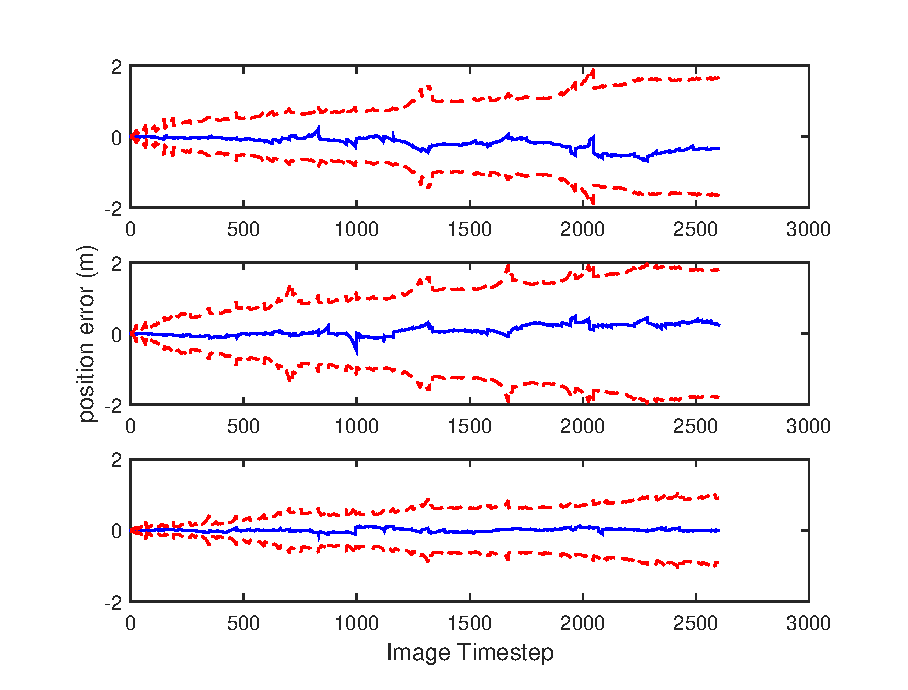
\includegraphics[scale=0.5]{position_error.eps}
	
	\caption{The position error (blue) and $ \pm 3 \sigma $ bounds (red) about axes x, y, and z. }
	\label{figurelabel}
\end{figure}

\begin{figure}[thpb]
	\centering
	
	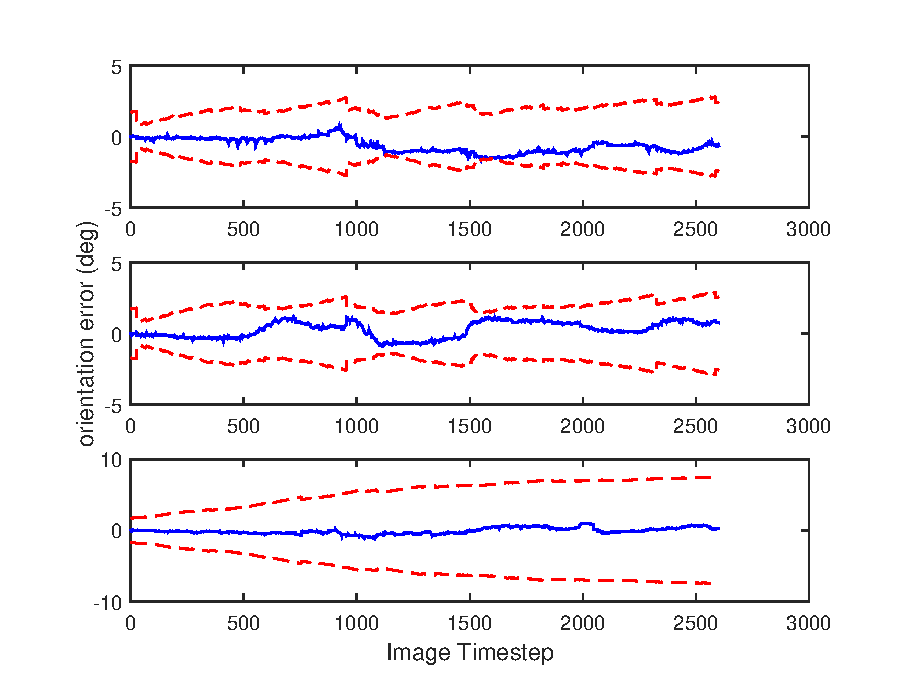
\includegraphics[scale=0.5]{orientation_error.eps}
	
	\caption{The orientation error (blue) and $ \pm 3 \sigma $ bounds (red) about axes x (roll), y (pitch), and z (yaw). }
	\label{figurelabel}
\end{figure}

\begin{figure*}[htbp] % Requires \usepackage{graphicx}
	\centering
	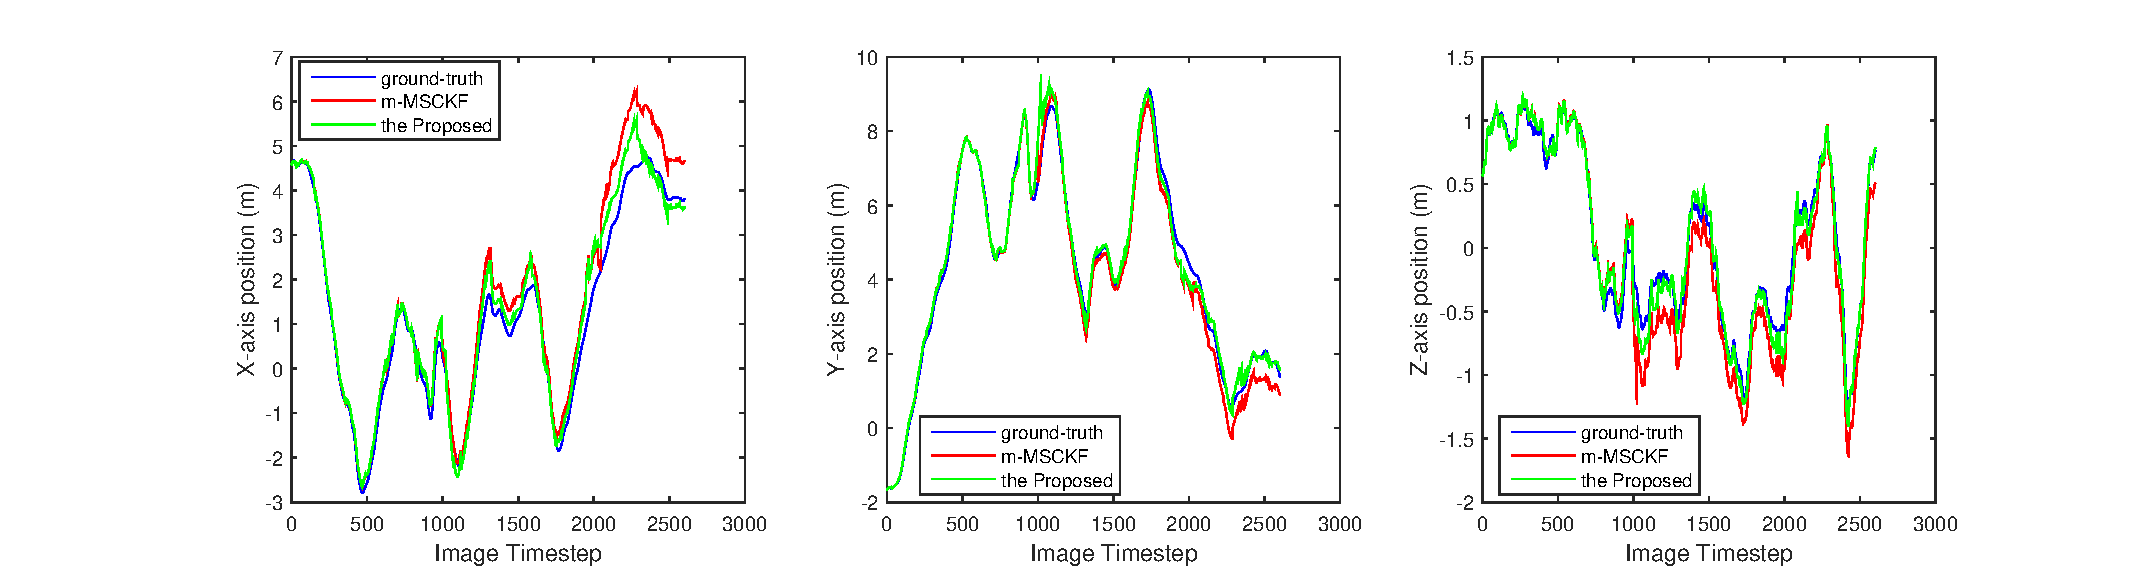
\includegraphics[width=1\linewidth]{3axis.eps} % 1\linewidth
	\caption{Experimental results: comparison of  ground-truth (blue), trajectories estimated by m-MSCKF (red) and the proposed method (green)}
	\label{fig2}
\end{figure*}

The results shown in Fig.3 and 4 show the error and $ \pm 3 \sigma $ bounds corresponding to position and orientation estimate. The plots reveal that the error remains bounded by $ \pm 3 \sigma $ , meaning that the filter is consistent. And the proposed estimator has correct observability properties for camera/IMU system. The roll and pitch are observable, the error bounds do not increase indefinitely.In contrast, those for the position and yaw do continuously increase because they are not observable \cite{kelly2011visual}.



In Fig.5, the estimated poses are displayed in X, Y and Z axis separately. It also gives a comparison between the m-MSCKF method. According to the ground truth, the final position is $ [3.8050 \ \   1.3780  \ \  0.7572]^T  $m. The final position estimation given by the m-MSCKF method is  $ [4.6609  \ \  0.9028    \ \ 0.5055]^T  $m, while the proposed method gives  $ [ 3.6275 \ \   1.5840  \ \  0.7833]^T  $m. The average error between the trajectory estimated by proposed method and the ground truth is $ [0.2810 \ \ 0.1804
\ \  0.0659]^T $m in three axis. The results show that the proposed method owns better  precision than m-MSCKF method.
 

 
 
\subsection{Sensors Calibration}

In order to validate the proposed filter algorithm is effective for estimating the IMU-camera transformation  while pose estimation, we added initial alignment error for translation and rotaion to the known extrinsic  calibration between sensors. 

For simplicity and due to limited space, in this section, we just discuss the calibration of transformation between IMU and CAM0. Because the calibration of IMU and CAM1 is in a similarity situation. The initial alignment error for translation is set to $ {\leftidx{^B}{\tilde  {\bm p}}_{C_0}} = [-0.03 \ \ 0.10 \ \ -0.09]^T $m with a  standard deviation of $ [0.0548 \ \   0.0447  \ \  0.0458]^T $m in each axis. The initial alignment error for rotation is set to $ \leftidx{_B^{C_0}} { \bm {\delta \theta}} = [5^{\circ} \ \ 6^{\circ} \ \ -4^{\circ}]^T $ with a standard deviation of  $ [3.3914^{\circ}  \ \  3.8455^{\circ}  \ \  3.1917^{\circ}]^T $ in each axis of rotation. Consequently, the filter state vector and
error-state covariance matrix are initialized according to the
process described in Section II.





In Figs.6 and 7, the  IMU-camera clibration errors and their $ 3 \sigma $ bounds for the
6-DOF transformation between the IMU and the camera are shown.

\begin{figure}[thpb]
	\centering
	
	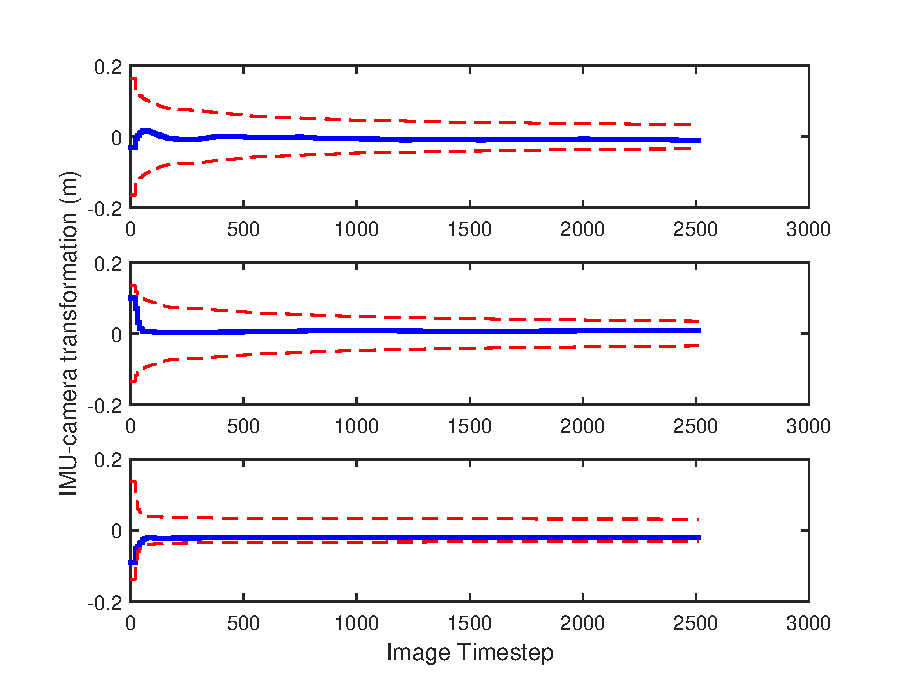
\includegraphics[scale=0.5]{trans.eps}
	
	\caption{IMU-camera translation error (blue) and $ 3 \sigma $ bounds (red). Translation along axes x, y, and z. }
	\label{figurelabel}
\end{figure}

\begin{figure}[thpb]
	\centering
	
	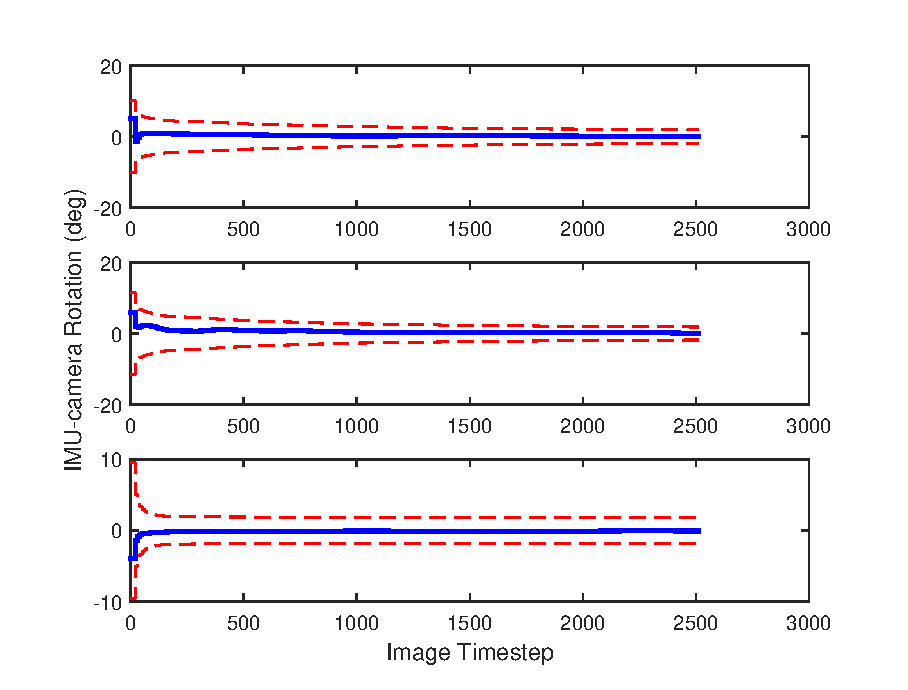
\includegraphics[scale=0.5]{rot.eps}
	
	\caption{IMU-camera rotation error (blue)and $ 3 \sigma $ bounds (red). Rotation about axes x (roll), y (pitch), and z (yaw). }
	\label{figurelabel}
\end{figure}

 Fianlly, we list the initial and final uncertanty of the IMU-camera parameters (transition and rotation), including CAM0 and CAM1 in Table I. The results shown here demonstrate that the proposed calibration is capable of operating in a real-world environment and this method is effective.



\section{CONCLUSIONS}
In this paper, we presented a filter-based visual inertial sensor fusion algorithm for pose estimation. The main contribution is the derivation of a measurement model of stereo visual observation. And no other method
of attempting to stereo visual information with inertial
sensor in a MSCKF framework has been found on literature yet. In addition, the proposed method estimates estrinsic calibration parameters between sensors to improve the performamce. The experimental results indicate that our method has a better accuracy than a self-implemented m-MSCKF ant it is effective to estimate sensor extrinsic calibration online.


\begin{table}
	\caption{FINAL UNCERTAINTY ($ 3 \sigma $) OF THE IMU-CAMERAS PARAMETERS AFTER 2500 IMAGE TIMESTEP}
	\label{multiprogram}
	\begin{center}
		\begin{tabular}{|c|c||c|c|c|c|c|c|}
			\hline
			\multicolumn{2}{|c||}{$ 3 \sigma $} & x(m) & y(m) & z(m) & r($ ^\circ $) & p($ ^\circ $) & y($ ^\circ $) \\
			\hhline{==#======}
			\multirow{2}{*}{CAM0}
			&Initial & 0.16 & 0.13 & 0.134 & 10.17  & 11.53 &   9.57 \\
			
			& Final & 0.03 &    0.03&    0.03 & 1.90&   1.82&    1.81\\
			\hhline{==#======}
			\multirow{2}{*}{CAM1}
			&Initial &0.28&    0.23&    0.19 &  9.41&   12.63&   12.06 \\
			
			&Final & 0.03 &   0.03&    0.03 & 1.90 &   1.83&    1.84 \\
			\hline
		\end{tabular}
	\end{center}
\end{table}



\addtolength{\textheight}{-12cm}   % This command serves to balance the column lengths
                                  % on the last page of the document manually. It shortens
                                  % the textheight of the last page by a suitable amount.
                                  % This command does not take effect until the next page
                                  % so it should come on the page before the last. Make
                                  % sure that you do not shorten the textheight too much.

%%%%%%%%%%%%%%%%%%%%%%%%%%%%%%%%%%%%%%%%%%%%%%%%%%%%%%%%%%%%%%%%%%%%%%%%%%%%%%%%



%%%%%%%%%%%%%%%%%%%%%%%%%%%%%%%%%%%%%%%%%%%%%%%%%%%%%%%%%%%%%%%%%%%%%%%%%%%%%%%%







%%%%%%%%%%%%%%%%%%%%%%%%%%%%%%%%%%%%%%%%%%%%%%%%%%%%%%%%%%%%%%%%%%%%%%%%%%%%%%%%




\bibliographystyle{IEEEtran}
\bibliography{robio}




\end{document}
